\chapter{Linearization algorithm}

\section*{Introduction}

\lpeq{} consists of 10 main phases:
\begin{enumerate}[1.]
\item Rewrite output values to input values.
\item Eliminate locally defined constants.
\item Eliminate of state automata (unsupported).
\item Create new processes for all sub-expressions of \pedi{} expressions, which are called `threads'; replace the sub-expressions themselves by instantiations of those processes.
\item Create new processes for each combination of channel parameters with which a process is instantiated (this is called `channel flattening').
\item Construct a process dependency tree from the model in order to confirm that the model does not contain parallel recursion.
\item Add a program counter to each process.
Associate all sequential expressions with a unique value of the program counter, and rewrite processes so that they become disjunctions of recursive process instantiations (typically in combination with an action prefix) and guarded \pedi{} expressions.
\item Rewrite processes so that all recursive process instantiations have an action prefix (this is called `prefix resolution').
\item Linearize \pedi{} expressions.
So far, this has only been implemented for the Parallel expression.
\end{enumerate}

The phases can also be found in Figure~\ref{main-flow:fig}.

\begin{figure}[!ht]
\begin{center}
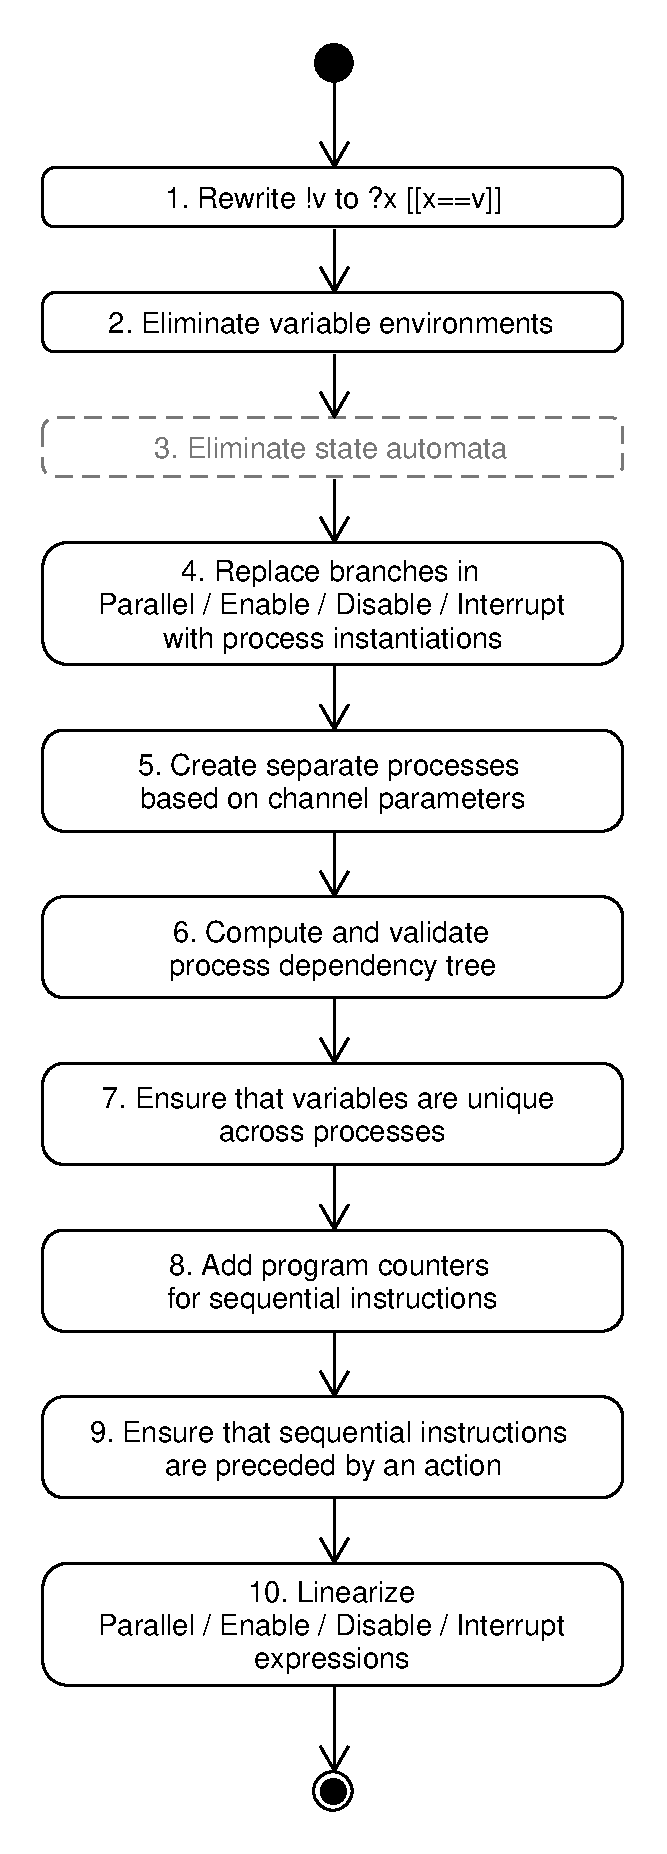
\includegraphics[width=0.5\linewidth]{umlet/linearization-main-flow}
\caption{Main flow.}
\label{main-flow:fig}
\end{center}
\end{figure}

\begin{samepage}
\section{Rewriting output values to input values}

\lpeq{} performs a depth-first search on the behavioral expression of the model.
When it encounters an action prefix $A$, it looks for all occurrences of the form $\texttt{!}v$ (where $v$ is an expression) in $A$.
For each occurrence, \lpeq{} does the following:
\begin{enumerate}[1.]
\item A fresh variable $x$ of the same sort as $v$ is introduced.
\item $\texttt{!}v$ is replaced by $\texttt{?}x$, the declaration of $x$.
\item $g_A$, the guard of $A$, is changed to $g_A \land x = v$.
\end{enumerate}
\end{samepage}

\section{Eliminating locally defined constants}

In the behavioral expressions of \txs{}, constants can be defined locally with a \texttt{LET} expression.
Such expressions are also called `variable environments'.

\lpeq{} eliminates \texttt{LET} expressions through substitution.

\section{Eliminating state-automaton expressions}

\lpeq{} cannot handle this yet.

\section{Instantiating threads} \label{thread-inst:section}

\pedi{} expressions include at least two sub-expressions.
These sub-expressions are considered to run concurrently, and are therefore called `threads'.
The root behavioral expression of the model is also classified as a thread.

For convenience (and for the computation of the process dependency tree in phase 6, described in Section~\ref{procdeptree:section}) \lpeq{} does the following for each thread:
\begin{enumerate}[1.]
\item A new process $P$ is created, with the thread expression as its body.
\item The sub-expression itself (at its original location) is replaced by the appropriate instantiation of $P$.
\end{enumerate}

\section{Flattening channels}

\txs{} processes refer to channels, but the actual channel instances that are used depend on the channel parameters that were used when they were instantiated.
To change this, \lpeq{} requires all combinations of actual channel instances with which processes are instantiated.

Consider a process instantiation $I$.
Within the context of this phase, the \emph{signature} of $I$ refers to the process that is instantiated by $I$ in combination with the actual channel instances that are passed as channel parameters (in order).

At the start of this phase, \lpeq{} performs a depth-first search for signatures on the behavioral expression of the model (this expression may have been changed by earlier phases).
\lpeq{} will only recurse into a process instantiation if it produced a new signature.

For each signature that was found, \lpeq{} does the following:
\begin{enumerate}[1.]
\item A new process $P$ is created, initially with the same body as the body of the process of the signature.
Instead of its original channel parameters \lpeq{} uses the actual channel instances of the model.
\item Each channel reference in $P$ is replaced by the corresponding actual channel instance from the signature.
\item Each process instantiation $I$ is replaced by an instantiation of the new process that corresponds with the signature of $I$.
\end{enumerate}

\lpeq{} only executes the third instruction after the first instruction has been executed for all signatures.

\section{Computing the process dependency tree} \label{procdeptree:section}

The \emph{process dependency tree} is a tree where each node has as a value a process $P$ and as branches the thread processes (see Section~\ref{thread-inst:section}) on which the \pedi{} expressions that occur in the body of $P$ depend.
The tree is computed by \lpeq{} with a straightforward depth-first search.

Note that a process dependency tree only contains thread processes: if a thread process can reach a \pedi{} expression by sequentially instantiating another process $P$ first, $P$ does not become a node of the tree.

The process dependency tree should be finite; otherwise, there may exist infinite parallel recursion in the model.
Infinite parallel recursion should be avoided because it may result in a situation where an action leads to infinitely many different states, violating one of the assumptions required for how \txs{} generates tests; and therefore \lpeq{} terminates with an error message when it detects that a process dependency tree is infinite.

\lpeq{} also takes the opportunity to check whether the model has no infinite sequential recursion: recursion where a process instantiates itself without doing an action prefix first.
Among others, the absence of such recursion is a prerequisite for the termination of phase 8 (see Section~\ref{prefix-resolution:section}).

\section{Adding sequential program counters}

\subsection{Ensuring variable freshness}

In this phase, \lpeq{} will `merge' different processes.
These processes may use the same variables for different purposes.
To avoid conflicts in a lazy but foolproof manner, \lpeq{} first rewrites all involved processes so that each data parameter and each communication variables only occurs once (across processes).

\subsection{Updating process signatures}

Second, \lpeq{} does the following for each thread process (see Section~\ref{thread-inst:section}) $P$:
\begin{enumerate}[1.]
\item It gathers all variables that are (recursively) used by $P$.
This includes both data parameters and communication variables, but \emph{not} variables from thread processes on which $P$ depends.
\item It creates a fresh data parameter $\textit{pc}$ of sort \texttt{Int}.
This parameter can be interpreted as the \emph{program counter} of $P$.
\item It defines a new signature for $P$ (in particular, it defines new data parameters for $P$), consisting of $\textit{pc}$ and all variables gathered in the first instruction.
\lpeq{} also maintains a record of how process instantiations should be changed in accordance with the new signature.
\end{enumerate}

\subsection{Flattening sequential expressions} \label{flattenseqexprs:section}

Third, \lpeq{} recurses through the behavioral expression of each thread process $P$.
Meanwhile, simply put, the following work happens:
\begin{itemize}
\item A body of disjunctive behavioral expressions (a \choice{} expression) is composed, starting with zero expressions.
\lpeq{} will convert and add each behavioral sub-expression of $P$, recursing into regular processes (if not visited before) but not into other thread processes.
Each addition to the body has an appropriate program counter value associated with it, and they can be reached by instantiating $P$ with that value.
\item Instantiations of thread processes are updated (they require the initial value of the program counter, which is always \texttt{0}).
\item Instantiations of regular processes are changed to instantiations of $P$.
Each regular process is visited only once, and \lpeq{} maintains a record of the program counter value that is associated with visiting that process so that other visits can make use of the same value later.
\item Occurrences of \texttt{STOP} are replaced by an instantiation of $P$ in which the program counter is set to $\texttt{-1}$.
\end{itemize}

\lpeq{} does the above tasks for thread processes in such an order that when work starts on a thread process $P$ all thread processes on which $P$ depends have already been through the same procedure.
\lpeq{} extracts the order from the process dependency tree (see Section~\ref{procdeptree:section}): thread processes with a larger maximum distance to the root of the tree are processed \emph{before} thread processes with a smaller maximum distance to the root of the tree.

\section{Resolving prefixes} \label{prefix-resolution:section}

Where possible, \lpeq{} makes the structure of thread processes more regular by ensuring that recursive process instantiations are preceded by action prefixes (\pedi{} expressions are left alone again).
This is accomplished by substitution: \lpeq{} essentially repeatedly replaces recursive instantiations of a thread process $P$ without a preceding action prefix by the body of $P$ until a situation is reached where all instantiations of $P$ are preceded by action prefixes.
This procedure terminates because the model does not contain infinite sequential recursion, a property that is established in phase 6 (see Section~\ref{procdeptree:section}).

\section{Linearizing expressions with threads}

\subsection*{Current state of the model}

By design, each thread process $P$ that is located on a leaf of the process dependency tree of the model in its current state is already (almost) linear: its body consists of a single \choice{} expression, and the choices consist of an action prefix followed by an instantiation of $P$, possibly nested in a \texttt{HIDE} expression.
Only the last part violates the requirements for linearity.

A thread process $Q$ that exists elsewhere in the process dependency tree is, of course, \emph{not} linear: even though its body consists of a single \choice{} expression, its choices can have two forms.
These forms are:
\begin{itemize}
\item An action prefix followed by an instantiation of $Q$, possibly nested in a \texttt{HIDE} expression (this form satisfies linearity except for the \texttt{HIDE} expression).
\item A guard followed by a \pedi{} expression, possibly nested in a \texttt{HIDE} expression.
It will take specific actions to linearize choices of this form, of which $Q$ contains at least one.
\end{itemize}

\subsection*{General flow}

For each thread process $P$, \lpeq{} does the following:
\begin{enumerate}[1.]
\item It separates choices with a \pedi{} expression from choices without a \pedi{} expression.
\item Choices without a \pedi{} expression are used as the start of a fresh body of $P$.
\item One by one, choices with a \pedi{} expression are linearized.
In preparation, \lpeq{} rewrites the thread processes on which a \pedi{} expression depends so that they no longer contain \texttt{HIDE} expressions.
Linearization of the \pedi{} expression results in a number of new choices that are added to the new body of $P$ that is being composed.
\item \lpeq{} checks that the final form of the new body of $P$ is indeed linear.
\end{enumerate}

\lpeq{} does the above tasks for thread processes in such an order that when work starts on a thread process $P$ all thread processes on which $P$ depends have already been through the same procedure.
\lpeq{} extracts the order from the process dependency tree (see Section~\ref{procdeptree:section}): thread processes with a larger maximum distance to the root of the tree are processed \emph{before} thread processes with a smaller maximum distance to the root of the tree.

A graphical overview of the procedure can also be found in Figure~\ref{pbranch-flow:fig}.
Each step is described separately in the remaining sections of this chapter.

\begin{figure}[!ht]
\begin{center}
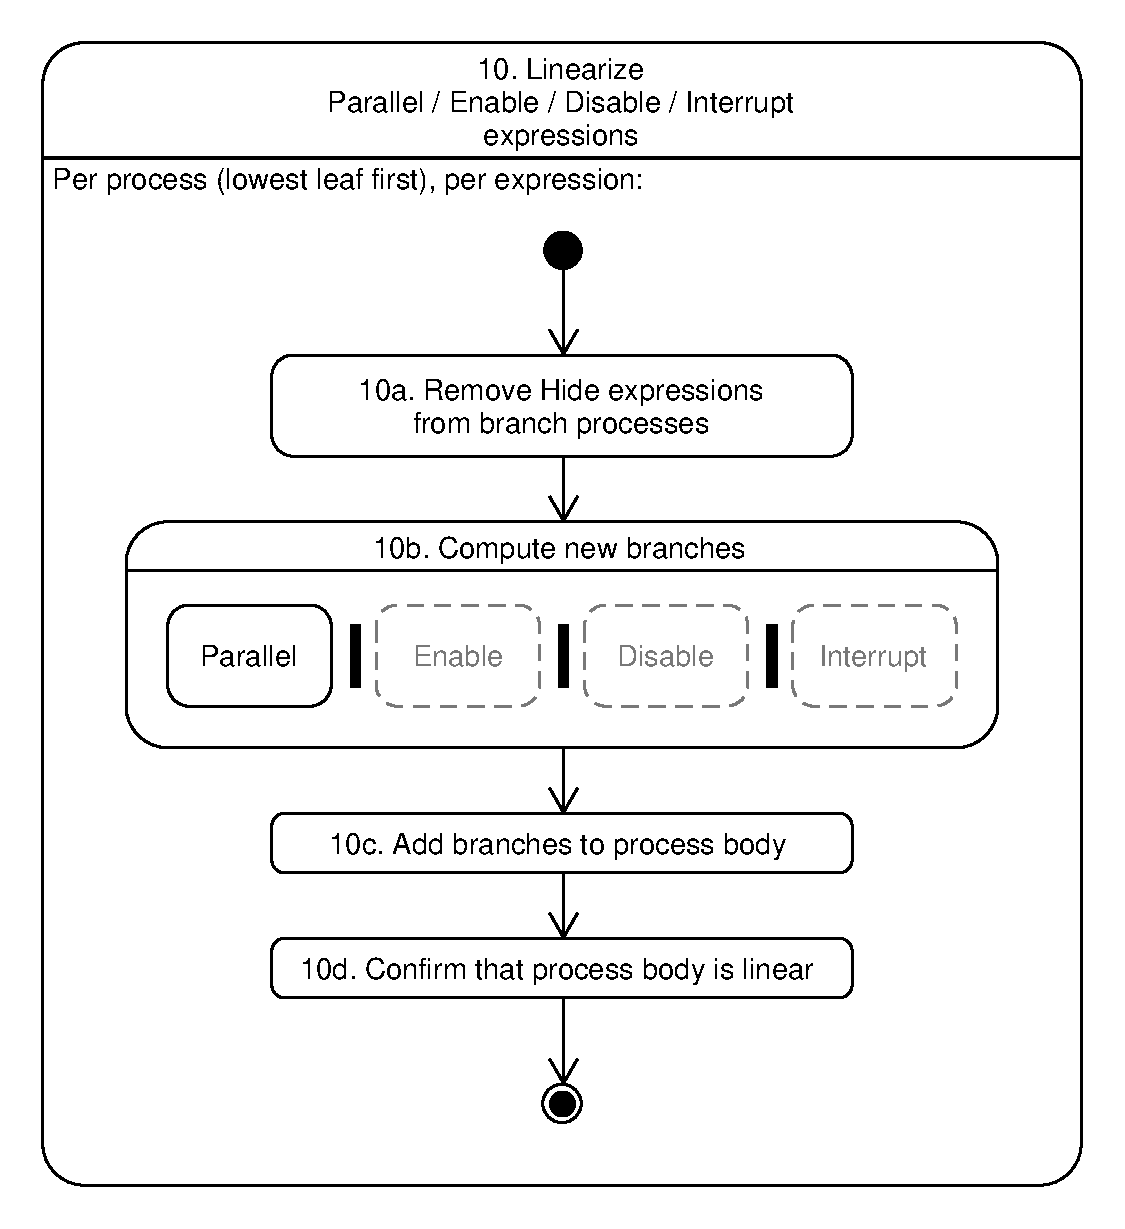
\includegraphics[width=0.8\linewidth]{umlet/linearization-pbranch-flow}
\caption{Flow for linearizing expressions with threads.}
\label{pbranch-flow:fig}
\end{center}
\end{figure}

\subsection{Eliminating Hide expressions}

\subsection{Linearizing Parallel}

\subsection{Linearizing Enable}

\subsection{Linearizing Disable}

\subsection{Linearizing Interrupt}



